% Poster copy of the report's SqueezeNet Fire drawing (R2): truth vs the fine-tuned 1.5B's reply.
% Build: pdflatex fig4_fire.tex  ->  copy fig4_fire.pdf to ../figures/
\documentclass[border=2pt]{standalone}
\usepackage[T1]{fontenc}
\usepackage{lmodern}
\usepackage{xcolor,tikz}
\usetikzlibrary{arrows.meta}
\definecolor{hiec}{HTML}{EB6834}
\definecolor{bad}{HTML}{E34948}
\newcommand{\demofont}{\fontsize{5.6}{6.3}\selectfont\ttfamily}
\tikzset{fx/.style={draw, rounded corners=1.5pt, font=\fontsize{5.4}{6}\selectfont, inner sep=1.4pt,
  minimum height=3.6mm, minimum width=6.5mm, fill=white},
  ar/.style={-{Stealth[length=3pt]}, line width=0.4pt}}
\begin{document}
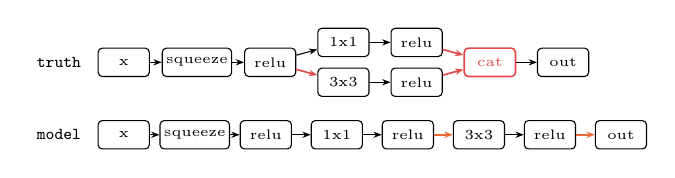
\begin{tikzpicture}[x=9.3mm, y=4.6mm]
\node[font=\demofont, anchor=east] at (-0.45,0) {truth};
\node[fx] (a0) at (0,0) {x}; \node[fx] (a1) at (1,0) {squeeze}; \node[fx] (a2) at (2,0) {relu};
\node[fx] (a3) at (3,0.55) {1x1}; \node[fx] (a4) at (4,0.55) {relu};
\node[fx] (a5) at (3,-0.55) {3x3}; \node[fx] (a6) at (4,-0.55) {relu};
\node[fx, draw=bad, text=bad, line width=0.6pt] (a7) at (5,0) {cat}; \node[fx] (a8) at (6,0) {out};
\foreach \a/\b in {0/1,1/2,2/3,3/4,5/6,7/8} \draw[ar] (a\a) -- (a\b);
\draw[ar, draw=bad, line width=0.6pt] (a2) -- (a5); \draw[ar, draw=bad, line width=0.6pt] (a4) -- (a7);
\draw[ar, draw=bad, line width=0.6pt] (a6) -- (a7);
\node[font=\demofont, anchor=east] at (-0.45,-2) {model};
\foreach \i/\l in {0/x,1/squeeze,2/relu,3/1x1,4/relu,5/3x3,6/relu,7/out}
  \node[fx] (b\i) at (\i*0.97,-2) {\l};
\foreach \a/\b in {0/1,1/2,2/3,3/4,5/6} \draw[ar] (b\a) -- (b\b);
\draw[ar, draw=hiec, line width=0.6pt] (b4) -- (b5); \draw[ar, draw=hiec, line width=0.6pt] (b6) -- (b7);
\end{tikzpicture}
\end{document}
